\documentclass[border=3pt]{standalone}
% Preâmbulo compartilhado pelos diagramas TikZ da aula 9 de IHR (Robôs na Sociedade)
\usepackage[T1]{fontenc}
\usepackage[utf8]{inputenc}
\usepackage{lmodern}
\usepackage{amsmath}
\usepackage{xcolor}
\usepackage{tikz}
\usetikzlibrary{arrows.meta,angles,quotes,decorations.pathmorphing,decorations.pathreplacing,calc,
                positioning,shapes.geometric,shapes.misc,backgrounds,fit,
                math}

% Paleta (mesma dos SVGs originais)
% Paleta da disciplina de IHR: acento azul (#1A6FB5), cor de destaque do tema.
% (o nome "dblue" é mantido para não alterar todos os diagramas)
\definecolor{dblue}{HTML}{1A6FB5}
\definecolor{dorange}{HTML}{B3541E}
\definecolor{dgreen}{HTML}{4A7C59}
\definecolor{dred}{HTML}{9C4B4B}
\definecolor{dcream}{HTML}{F4F1EA}
\definecolor{dshade}{HTML}{DDD7C9}

% Função gaussiana (não normalizada por padrão de escala visual)
\pgfmathdeclarefunction{gauss}{3}{%
  \pgfmathparse{1/(#3*sqrt(2*pi))*exp(-((#1-#2)^2)/(2*#3^2))}%
}

% Estilos comuns (prefixo d... para não colidir com chaves internas do pgf)
\tikzset{
  >={Stealth[length=2mm]},
  dguide/.style={gray!55, dashed, line width=0.4pt},
  daxis/.style={gray!60, line width=0.7pt, ->},
  dbody/.style={fill=black!3, draw=black!80, line width=1pt},
  dacc/.style={draw=dblue, line width=1pt},
  dlbl/.style={black!55, font=\small},
  dsub/.style={black!45, font=\footnotesize},
  dstate/.style={circle, draw=black!80, fill=dcream, line width=1pt,
                 minimum size=17mm, font=\large, inner sep=1pt},
  dobs/.style={circle, draw=black!80, fill=dshade, line width=1pt,
               minimum size=14mm, font=\large, inner sep=1pt},
  dbox/.style={rounded corners=2pt, draw=black!80, fill=dcream, line width=1pt,
               align=center, inner sep=6pt},
  dop/.style={circle, draw=black!80, fill=white, line width=1pt,
              minimum size=6mm, inner sep=0pt, font=\small},
  dtrans/.style={->, dblue, line width=1pt},
  dmeas/.style={->, dorange, line width=1pt},
  dcurve/.style={line width=1pt, dblue},
  dcurveb/.style={line width=1.4pt, dorange},
}

\begin{document}
\hyphenpenalty=10000 \exhyphenpenalty=10000 \tolerance=9999 \emergencystretch=3em
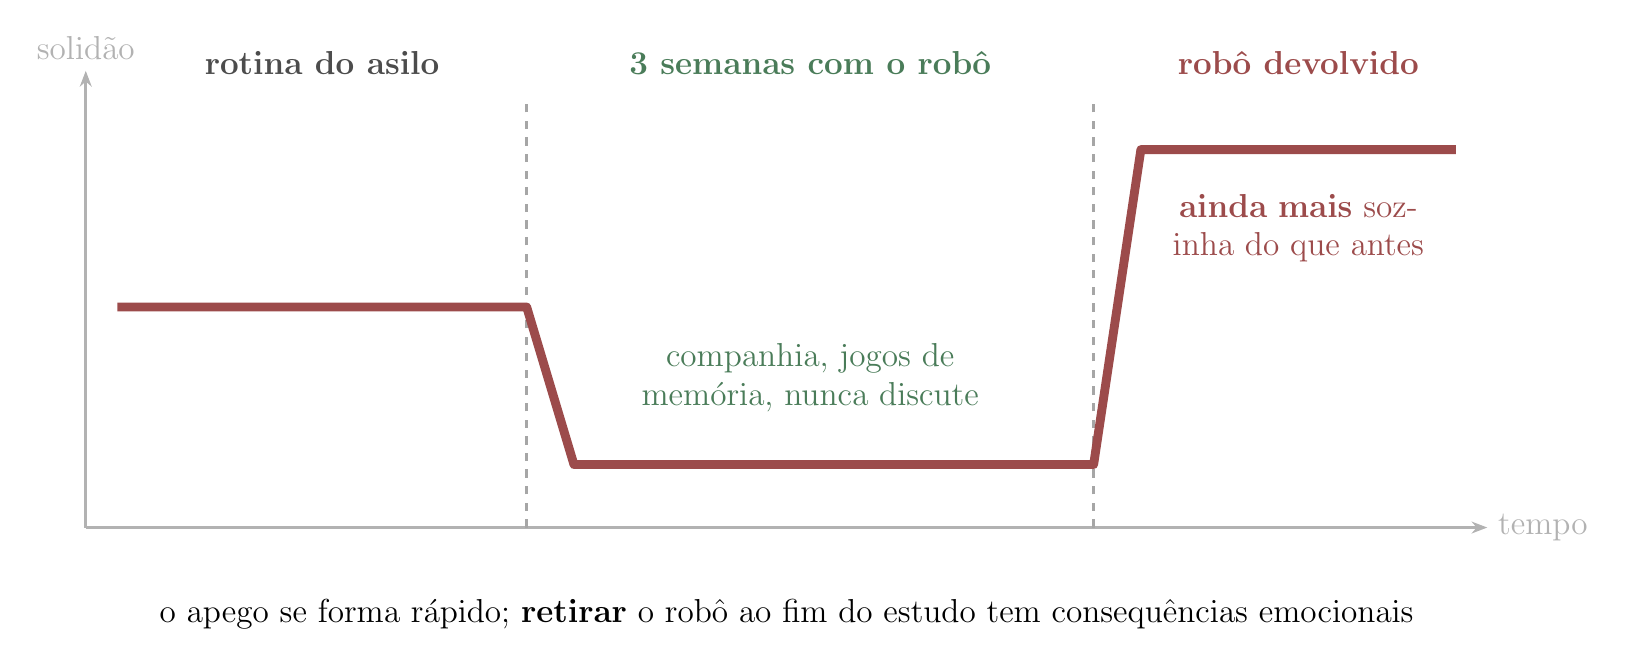
\begin{tikzpicture}[x=1cm,y=1cm]
\draw[daxis, line width=1.2pt] (0.8,1.6) -- (18.6,1.6) node[right, font=\large] {tempo};
\draw[daxis, line width=1.2pt] (0.8,1.6) -- (0.8,7.4) node[above, font=\large] {solidão};
\draw[black!35, dashed, line width=1.1pt] (6.4,1.6) -- (6.4,7.0);
\draw[black!35, dashed, line width=1.1pt] (13.6,1.6) -- (13.6,7.0);
\draw[dred, line width=3.2pt, line join=round] (1.2,4.4) -- (6.4,4.4) -- (7.0,2.4) -- (13.6,2.4) -- (14.2,6.4) -- (18.2,6.4);
\node[font=\large\bfseries, black!70, text width=5cm, align=center] at (3.8,7.5) {rotina do asilo};
\node[font=\large\bfseries, dgreen, text width=7cm, align=center] at (10.0,7.5) {3 semanas com o robô};
\node[font=\large\bfseries, dred, text width=4.4cm, align=center] at (16.2,7.5) {robô devolvido};
\node[font=\large, dgreen, text width=6.4cm, align=center] at (10.0,3.5) {companhia, jogos de memória, nunca discute};
\node[font=\large, dred, text width=4.4cm, align=center] at (16.2,5.4) {\textbf{ainda mais} sozinha do que antes};
\node[font=\large, text width=18cm, align=center] at (9.7,0.5) {o apego se forma rápido; \textbf{retirar} o robô ao fim do estudo tem consequências emocionais};
\end{tikzpicture}
\end{document}
